\documentclass[msc,proposal,hidelot,hideabstract]{ppgccufmg} % ou [msc] para dissertações
                                        % de mestrado. Para propostas ou
                                        % projetos, usar [phd,project],
                                        % [msc,proposal], etc.
\usepackage[brazil]{babel} % ajusta vários detalhes para
                           % documentos escritos em português,
                           % principalmente hifenização
\usepackage[T1]{fontenc}   % permite a hifenização de
                           % palavras acentuadas
\usepackage[utf8x]{inputenc} % ou [utf8x] para quem prefere
                             % usar a codificação UTF-8
\usepackage{graphicx} % define o comando \includegraphics
                      % para a inclusão de Figuras
%\usepackage[square]{natbib} % permite citações naturalmente
                            % integradas ao texto
\usepackage[a4paper,
portuguese,
bookmarks=true,
bookmarksnumbered=true,
linktocpage,
colorlinks=true,
citecolor=black,
urlcolor=black,
linkcolor=black,
filecolor=black,
]{hyperref}
\usepackage[table,xcdraw]{xcolor}
\usepackage{amsmath}
\begin{document}
\ppgccufmg{
title={Um estudo de ferramentas de \\
Suporte de Problemas de Software},
author={Vagner Clementino dos Santos},
university={Universidade Federal de Minas Gerais},
course={Ciência da Computação},
address={Belo Horizonte},
date={2015-11},
advisor={Rodolfo F. Resende},
abstract={Resumo}{resumo},
}
\chapter{Introdução}
\label{ch:intro}
Dentro do ciclo de vida de um produto de software o processo de manutenção tem
papel fundamental. Devido ao seu alto custo, em alguns casos chegando em 60\%
do custo total do software \cite{kaur2015review}, este processo deve ter sua
importância considerada tanto pela comunidade científica quanto pela indústria.

\textit{Manutenção} pode ser definida como o processo de modificar um componente ou um
sistema de software após a sua entrega a fim de corrigir falhas, melhorar o desempenho ou outro atributo, ou adaptá-lo para mudanças ambientais
\cite{{159342}}. De outra forma, \textit{Manutenibilidade} é a propriedade de um
sistema ou componente de software com relação ao grau de \textit{facilidade}
em que ele pode ser corrigido, melhorado ou adaptado \cite{{159342}}.

As manutenções em software podem ser divididas em Corretiva, Adaptativa, Perfectiva e Preventiva \cite{Lientz:1980:SMM:601062,159342}. A
Manutenção Corretiva lida com a reparação de falhas encontradas. A Manutenção
Adaptativa têm o foco na adaptação do software devido à mudanças ocorridas no
ambiente em que ele está inserido. A Manutenção Perfectiva trabalha com
a modificação de um produto de software com o objetivo de detectar e corrigir
falhas latentes antes que elas se manifestem como tal. A Manutenção
Perfectiva fornece melhorias na documentação, desempenho e na manutenibilidade,
dentre outros atributos do sistema. A Manutenção Preventiva se preocupa com atividades
que possibilitem aumento da manutenibilidade do sistema. A \textit{ISO 14764}
\cite{1703974} propõe a divisão da tarefa de manutenção nos quatros tipos
descritos anteriormente e agrupa-os em termo único denominado
\textit{Requisição de Mudança - Modification Request (RM)}, conforme pode ser
visto pela Figura \ref{fig:modification-request}

\begin{figure}[hbtp]
\centering
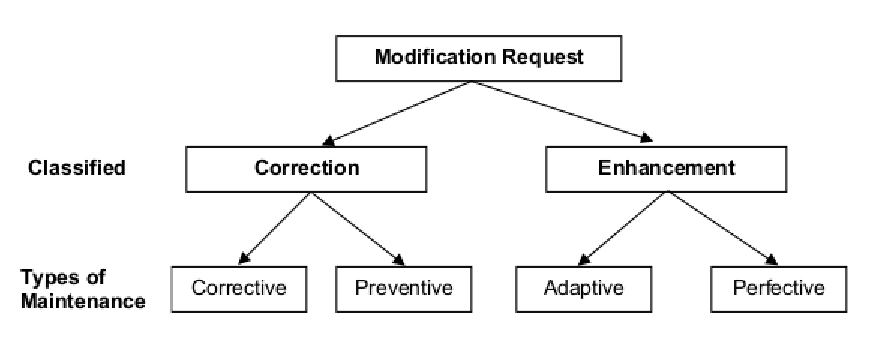
\includegraphics[width=.75\textwidth]{../img/modification_request.eps}
\caption{Tipos de manutenção segundo a norma ISO/IEC 14764. Extraído de
  \cite{1703974}}
\label{fig:modification-request}
\end{figure}

Em um ambiente real de desenvolvimento e manutenção de software, independente do tipo
de Requisição de Mudança a ser tratada, existe a necessidade de
gerenciar as RM's, especialmente por conta do seu volume. Esse controle é geralmente realizado
por Sistemas de Controle de Demandas (SCD)- Issue Tracking Systems  que ajudam
os desenvolvedores na correção de forma individual ou colaborativa de defeitos (bugs) ou
ainda na implementação de novas funcionalidades. Verifica-se na literatura diversos
sinônimos para os Sistemas de Controle de Demanda (Sistema de Controle de
Defeitos - Bug Tracking Systems, Sistema de Gerenciamento da Requisição -
Request Management System e outros ), todavia, de modo geral, o
termo se refere as ferramentas utilizadas pelas organizações para \textit{suporte de problemas de software}. Os SCD's são também utilizados por gestores, analistas de qualidade e usuários finais para
tarefas tais como gerenciamento de projetos, comunicação, discussão e revisões
de código. A maioria desses sistemas são projetados em torno do termo "demanda"
(bug, defeito, bilhete, recurso, etc.), contudo, cada vez mais este modelo parece
ser distante das necessidades práticas dos projetos de software
\cite{Baysal:2013:SAP:2486788.2486957}.

A manutenção de software muitas vezes aparece ligada aos processos tradicionais
de desenvolvimento de software. Existe o mito de que os métodos ágeis estão
principalmente concentrados na fase de desenvolvimento
\cite{kajko2009model}. No entanto, especialistas em software cada vez mais
avaliam que práticas ágeis podem ser adaptadas à evolução do software. Isso não
é totalmente surpreendente, já que métodos ágeis enfatizam a importância das
pessoas, o desenvolvimento incremental, a redução de riscos, e teste contínuo -
fatores que contribuem para a evolução e manutenção  eficaz de um software
\cite{thomas2006agile}. Desta forma tanto em um contexto que utilize processo de manutenção
``tradicional'' ou em que se aplique métodos ágeis pode-se tirar proveito das
SCD's para um melhor desempenho das atividades de manutenção.

Neste trabalho de dissertação vamos elaborar um Modelo Conceitual de Referência
dos Sistemas de Controle de Demandas (SCD) ao mesmo tempo em que iremos discutir os aspectos que
são considerados mais importantes do ponto de vista da literatura, bem como a partir de pontos de vistas de alguns
profissionais. De forma particular vamos estudar os mecanismos de
extensão que algumas destas ferramentas permitem. A partir dos resultados destas avaliações, caso o esforço seja
compatível com os prazos e recursos disponíveis, queremos elaborar extensões (plugins)
para uma ou mais (plugin) com o objetivo de apresentar e discutir nossa experiência.

Esta proposta de dissertação está estruturada da seguinte forma: o  Capítulo
\ref{ch:justificativa} discute a relevância deste trabalho no contexto da Engenharia de Software em especial no processo de Manutenção de
Software. O Capítulo \ref{ch:revisao} revisa a literatura com relação aos
trabalhos desenvolvidos sobre Manutenção de Software; é dado um foco especial
nos estudos que focam nos Sistemas de Controle de Demanda. No
Capítulo \ref{ch:metodologia} é discutida a metologia a ser aplicada visando a
elaboração do trabalho. No Capítulo \ref{ch:conclusao_trab_futuros} é apresentado o cronograma de
atividades da dissertação através da Tabela \ref{tab:cronograma}.

\chapter{Justificativa}
\label{ch:justificativa}
%Desde o final da década de 1970 \cite{Zelkowitz:1979:PSE:578504} percebe-se o aumento do custo referente as
%atividades de  manutenção de software. Nas décadas de 1980 de 1990 alguns
%trabalhos tiveram seu foco no desenvolvimento de modelos de mensuração do custo
%para manter o software \cite{Herrin:1985:SMC:323287.323383,hirota1994approach}.
%Na Tabela \ref{tab:software-cost}, adaptada de  \cite{koskinen2003software},
%é possível verificar esta tendência.
Diante da maior presença de software em todos os setores da sociedade
existe um interesse por parte da academia e da industria no desenvolvimento de
processos, técnicas e ferramentas que reduzam o esforço e o custo das tarefas
de desenvolvimento de software em geral e das atividades de manutenção em
particular. Neste linha verificamos o desenvolvimento de alguns trabalhos com
esta finalidade. Por exemplo, no trabalho de Yong \& Mookerjee \cite{1423995}  exite a proposição
de um modelo que reduz o custos de manutenção e reposição durante a vida útil de um sistema de software. O modelo
proposto demonstrou quem em algumas situações é \textit{melhor substituir um
  sistema do que mantê-lo}. Em outros estudos há menção de que o custo de
manutenção pode chegar a 60\% do custo total do software \cite{kaur2015review}. Este mesmo percentual
refere-se ao total de desenvolvedores dedicados à tarefas de manutenção de
sistemas \cite{Zhang_2003}.

A manutenção não necessariamente exige que o processo de software envolvido
seja o tradicional. Percebe-se alguns exemplos de adoção das práticas ágeis
para fins de manutenção e evolução do software \cite{kajko2009model}. Tal
tendência não é surpreendente tendo em vista que métodos ágeis enfatizam
características úteis, tais como desenvolvimento incremental e teste contínuo
que agregam valor para a evolução e manutenção eficaz de um software
\cite{thomas2006agile}.

O desenvolvimento e a manutenção de software envolve diversos tipos de métodos,
técnicas e ferramentas. Em especial no processo de manutenção, um aspecto
importante são as diversas Requisições de Mudanças que devem ser
gerenciadas. Este controle é realizado pelos Sistemas de Controle de Demandas(SCD) cujo uso vêm crescendo em importância sobretudo
por sua utilização por gestores, analistas da qualidade e usuários finais para
atividades como tomada de decisão e comunicação, dentre outras.

A utilização de  ``demanda'' como conceito central para as as ferramentas de
suporte de problemas de software parece ser distante das necessidades práticas dos projetos de software, especialmente
no ponto de vista dos desenvolvedores \cite{Baysal:2013:SAP:2486788.2486957}. Um exemplo deste desacoplamento do
SCD's com a necessidade de seus usuários pode ser visto no trabalho proposto por Baysal \& Holme \cite{baysal2012qualitative} no qual desenvolvedores que utilizam o Bugzilla\footnote{\url{https://www.bugzilla.org}} relatam a
dificuldade em manter uma compreensão global das RM's em que eles estão
envolvidos. Segundo os desenvolvedores seria interessante que a ferramenta
tivesse um suporte melhorado para a Consciência Situacional - Situational
Awareness, ou seja, eles gostariam de estar cientes da situação global do
projeto bem como das atividades que outras pessoas estão realizando. Um outro
sinal da necessidade de evolução do SCD's pode ser observado considerando as diversas extensões (plugins) propostos na literatura \cite{101186,Thung:2014:BIT:2635868.2661678,Kononenko:2014:DED:2591062.2591075}

Diante do exposto, é proposto neste projeto de dissertação a elaboração de um
\textit{Modelo Conceitual de Referência} dos Sistemas de Controle de Demandas. Vamos discutir os aspectos que são
considerados mais importantes do ponto de vista da literatura da área bem como
a partir de pontos de vistas de alguns profissionais. De forma particular vamos
estudar os mecanismos de personalização que algumas destas ferramentas permitem
e tentaremos ainda criar exemplos de personalização para alguma possível
extensão a ser identificada ao longo do trabalho.

%\begin{table}[ht]
%\resizebox{\textwidth}{!}{%
%\begin{tabular}{|c|c|c|c|}
%\hline
%\rowcolor[HTML]{FFFFFF}
%\textbf{Ano} & \textbf{Proporção} & \multicolumn{1}{c|}{\cellcolor[HTML]{FFFFFF}\textbf{Metodologia}} & \multicolumn{1}{c|}{\cellcolor[HTML]{FFFFFF}\textbf{Referência}} \\ \hline
%2000 & \textgreater90\% & $\frac{\text{(Custo com manutenção e evolução do software)}}{\text{(Custo total do software)}}$ &\cite{846201} \\ \hline
%1993 & 75\% & $\frac{\text{(Manutenção de Software)}}{\text{(Orçamento com Sistemas de Informação)}}$ & \cite{swe.cost.legacy2}\\ \hline
%1990 & \textgreater90\% & $\frac{\text{(Custo com manutenção de sistema)}}{\text{(Custo total com Software)}}$ & \cite{moad1990maintaining}\\ \hline
%1988 & 60-70\% & $\frac{\text{(Manutenção de software)}}{\text{(Orçamento com a operação de Sistemas de Gerenciamento da Informação)}}$ & \cite{Port1988}\\ \hline
%1984 & 65-75\% & $\frac{\text{(Esforço gasto em manutenção de software)}}{\text{(Tempo total disponível para esforço em Engenharia de Software)}}$ & \cite{McKee:1984:MFD:1499310.1499334}\\ \hline
%1981 & 50\% & $\frac{\text{(Tempo gasto com manutenção de software)}}{\text{(Tempo Total)}}$ & \cite{Lientz:1981:PAS:358790.358796}\\ \hline
%1979 & 67\% & $\frac{\text{(Custo com Manutenção)}}{\text{(Custo Total com Software)}}$ & \cite{Zelkowitz:1979:PSE:578504}\\ \hline
%\end{tabular}
%}
%\caption{Proporção do Custo de Manutenção de Software. Adaptado de \cite{koskinen2003software}}
%\label{tab:software-cost}
%\end{table}
%

%Uma possível forma de reduzir o custo de manutenção de um sistema de software é
%aumentar a produtividade do desenvolvedor devotado às atividade de
%manutenção. No contexto do processo de desenvolvimento de software tradicional,
%conforme supõe a \textit{ISO/IEC 14764} \cite{1703974}, a manutenção de
%software pode estruturada conforme a Figura \ref{fig:maintence-process}.
%
%\begin{figure}[hbtp]
%\centering
%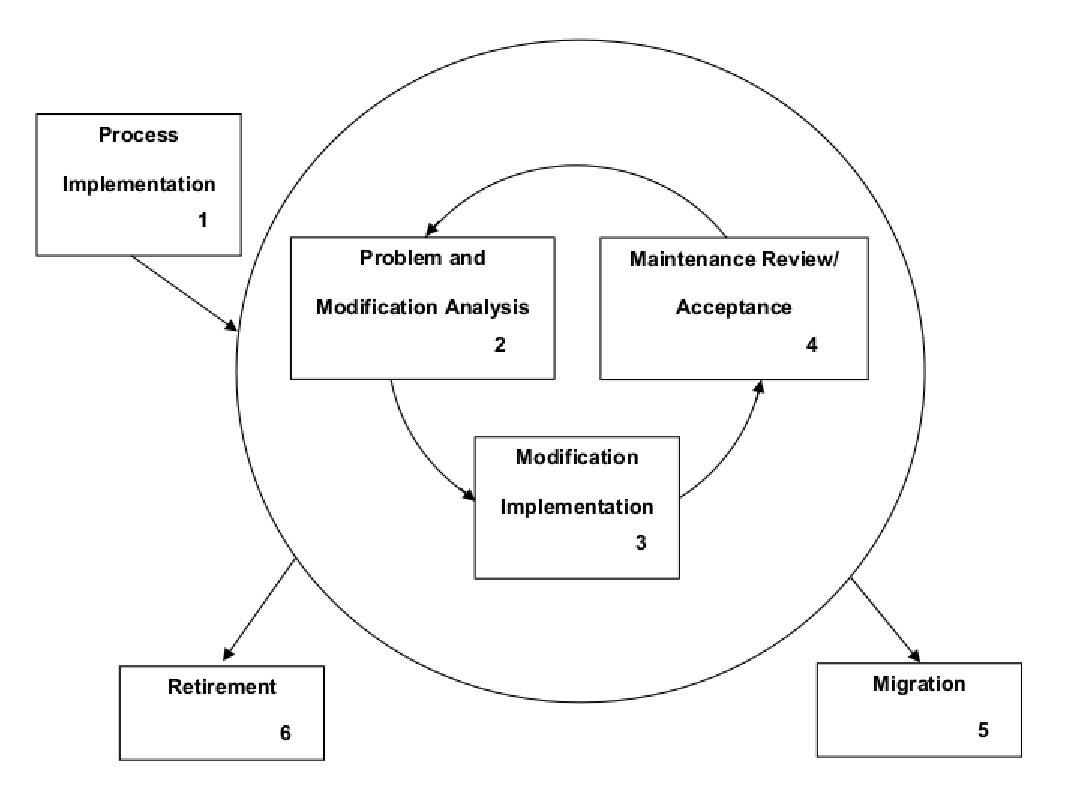
\includegraphics[width=.75\textwidth]{../img/maintence_process.eps}
%\caption{Processo de manutenção de software da norma ISO/IEC 14764. Adaptado: \cite{1703974}}
%\label{fig:maintence-process}
%\end{figure}
%
%Na atividade \textit{1 - Implementação do processo (Process
%Implementation)} os planos e procedimentos a serem executados
%durante a fase de manutenção devem ser estabelecidos e aprovados. Muitos o
%plano proposto define o processo de atribuição das MR's para os
%desenvolvedores. Esta tomada de decisão geralmente leva em conta a prioridade
%do serviço a ser realizado, as habilidades do programador dentre outros
%critérios. Todavia, este processo poderia obter melhores resultados se a cada
%Requisição atribuída a um desenvolvedor, outras similares, também pudessem ser
%sugeridas.
%
%
%Tal tomada de decisão apoiada por alguma metodologia para recomendar MR's
%similares trará os seguinte benefícios:
%
%\begin{itemize}
%\item \textit{Redução da troca de contexto (context switch)};
%\item \textit{Aumento da produtividade};
%\item \textit{Melhorar a qualidade das MR's sugeridas através de uma técnica mais
%  potente do que aquelas da Recuperação da Informação}.
%\end{itemize}
%%
%Com o objetivo de mensurar o cuto relativo à manutenção de software%
%\cite{benaroch2013primary,587341,ren2011research}, bem com melhoria as%
%atividades relacionadas ao procsso de manutenção  mediante a proposição%
%de modelos \cite{April200973}, cite{930170} e \cite{5741246} diversos%
%trabalhos vêm sendo propostos. esta mesma linha de pesquisa, alguns estudo%
%focam na melhoria da produtividde do desenvolvedor através de ações como a remoção de Requisições de Mudança -%
%Modification Request (MR) dupliadas%
%\cite{Alipour:2013:CAT:2487085.487123,6671283,09639314} ou ainda recomendando%
%MR's similares que reduzem a muança de contexto (context switch) \cite{5741246,101186}.%
%%
%Em geral, afim de remover dupiadas ou sugerir MR's similares são utilizadas de%
%técnicas de Recuperação da Infomação - Information Retrieve%
%\cite{baeza1999modern} tomando omo base a descrição textual da Requisição \cite{101186,Runeson:2007:DDD:1248820.1248882}. Apesar dos resultados%
%relevantes obtidos por esta técica verifica-se que ela é fortemente%
%dependente da forma que o solictante da MR descreve a sua requisição. Além disso%
%há problema dos sinônimos, em qe demandas similares mas, escritas com palavras%
%diferentes, podem não ser recupradas.%
%%
%Neste contexto é proposto umafrramenta para recomendação de Requisições de%
%Mudanças similares utilizando Rdes Neurais.%
%%
%O problema de recomendar Requsções de Mudanças similares pode ser definido%
%formalmente conforme segue:%
%%
%eja $I$ o conjunto de Requisçes de Mudanças (MR) em aberto para um%
%sistema $S$ qualquer. A cardinaidade de $I$ é dada por $n$. Seja $i$ um MR,%
%tal que $i \in I$, que foi atriuída para um desenvolver%
%$d$. Pede-se que seja encontrad um subconjunto $J \subset I$, de tamanho $k \ll n$, tal%
%que para todo $j$, tal que $j \n J$, seja similar a $i$ em um grau maior ou igual a%
%$s$. Onde $s$ é limiar inferiorde similaridade. Neste caso, o problema se resume em%
%encontrar uma função de similardade a ser aplicada a cada elemento $m \in I$,%
%onde $m \neq i$.%
%
\chapter{Revisão da Literatura}
\label{ch:revisao}

Uma tendência natural do software é evoluir a fim de atender novos requisitos ou alterações no ambiente no qual ele está inserido. Em uma séria de
estudos Lehman et al. propõe um conjunto de leis sobre a evolução do software. Dentre elas podemos destacar as leis da Mudança Contínua (Continuing
Change) e da Complexidade Crescente (Increasing complexity). Segundo a lei da
Mudança Contínua um programa que é utilizado em um ambiente real necessariamente deve mudar ou se tornará
progressivamente menos útil \cite{lehman1980understanding}. A lei da
Complexidade Crescente (Increasing complexity) afirma que quando um sistema em
evolução muda, sua estrutura tende a ser tornar mais complexa. Nesta situação
recursos extras devem ser disponibilizados a fim de preservar e simplificar a
estrutura do software \cite{lehman1980understanding}. As leis de Lehman têm
sido validadas, especialmente aquelas relacionadas a tamanho e
complexidade do software. Em um trabalho recente Yu \& Mishra \cite{{yu2013empirical}} examinaram e avaliaram de forma empírica
as Leis de Lehman com relação a evolução da qualidade do software. Os
resultados dão suporte as Leis de Lehman especialmente a que versa sobre a qualidade
do software onde declara-se que um produto de software decresce a sua qualidade ao
longo do tempo, exceto que ele seja reestruturado.

Percebida a importância do processo de manutenção de software, alguns trabalhos foram propostos visando mensurar o seu custo bem como propor
processos visando a redução do esforço envolvido neste tipo de atividade.

No trabalho de Herrin \cite{Herrin:1985:SMC:323287.323383} foi proposto um modelo matemático com o
objetivo de avaliar o impacto financeiro no orçamento de uma universidade das atividades de manutenção no sistema
de processamento de dados da instituição. O modelo propõe que o valor disponível para desenvolvimento de um novo sistema é
função inversa do custo de manutenção do software existente. Desta forma, o
fato de se manter um sistema durante muito tempo poderá impossibilitar a aquisição ou mesmo o desenvolvimento de um novo sistema.

No estudo de Hirota et al. \cite{hirota1994approach} é proposta a utilização de
da técnica Análise de Ripple para predizer o custo da manutenção de software. O
termo ``efeito Ripple'' foi utilizado pela primeira vez em um artigo publicado
por Haney \cite{haney1972module} e descreve a forma que a mudança em um módulo poderia
necessariamente causar alterações em outras partes do sistema
\cite{bilal2005using}. A Análise Ripple é uma forma de analisar informações de fluxo de dados das variáveis
dentro de um determinado contexto de um programa. Os valores retornados pela
aplicação da técnica são denominados Complexidade de Ripple. Os resultados
demostraram que a Complexidade de Ripple está mais relacionada ao entendimento do
software do que as métricas padrão, como linhas de código, complexidade
ciclomática e pontos de função. Desta forma, a Complexidade de Ripple poderia ser
utilizada para predizer os custo de manutenção de um sistema.

Mediante o uso de Redes Neurais Shula \& Misra
\cite{Shukla:2008:ESM:1342211.1342232} propõe um estudo para medir o custo de
manutenção de software. O trabalho discute a utilização de outras métricas além
de linha de código ou pontos de função para medir o tamanho e o custo do
processo de manutenção. Os resultados demonstraram a possibilidade de
construção de um modelo de mensuração de custo utilizando Redes
Neurais. Contudo, os resultados são sensíveis a escolha da arquitetura e
parâmetros de treino, os quais idealmente deveriam ser preparados por um
especialista no sistema a ser avaliado.

Diante da crescente importância dos Sistemas de Controle de Demandas no processo de manutenção de software, diversos
trabalhos vêm sendo propostos com o objetivo de entender como eles estão sendo
utilizados na prática e sugerir melhorias no desenho para desenvolver futuros SCD's.

No trabalho de Junio et al. \cite{5741246} é proposto um processo denominado PASM (Process for Arranging
Software Maintenance Requests) que propõe lidar com tarefas de manutenção como
projetos de software. Para tanto, utilizou-se técnicas de análise de
agrupamento (clustering) a fim de melhor compreender e comparar as demandas de
manutenção. Os resultados demostraram que depois de adotar o PASM os
desenvolvedores têm dedicado mais tempo para análise e validação e menos tempo
para as tarefas de execução e de codificação.

No estudo realizado por Bettenburg et al. \cite{bettenburg2008makes} foi
desenvolvida uma pesquisa (\textit{survey}) entre desenvolvedores e usuários dos
projetos Apache\footnote{\url{http://www.apache.org/}},
Eclipse\footnote{\url{https://www.eclipse.org}} e
Mozilla\footnote{\url{https://www.mozilla.org}} a fim de verificar o que
produziria um bom Sistema de Controle de Demanda. Os resultados demonstraram
que do ponto de vista dos desenvolvedores foram consideradas úteis
funcionalidades tais como reprodução do erro, rastros de pilhas (stack traces) e casos de
testes. A partir deste resultado foi construído um protótipo de um SCD
capaz de conduzir os usuários na coleta e fornecimento de um maior número de
informações úteis para a resolução do defeito reportado.

Avaliando o controle de demandas como um processo social, Bertram et
al. \cite{Bertram:2010:CCB:1718918.1718972} realizaram um estudo qualitativo em
SCD's quanto utilizados por pequenas equipes de desenvolvimento de software. Os resultados mostraram que um SCD não é apenas um
banco de dados de rastreamento de defeitos, recursos ou pedidos de informação, mas
também atua como um ponto focal para a comunicação e coordenação para diversas
partes interessadas (stakeholders) dentro e fora da equipe de software. Os
clientes, gerentes de projeto, o pessoal envolvido com a garantia da qualidade
e programadores, contribuem em conjunto para o conhecimento compartilhado dentro do contexto dos SCD's.

Em Zimmermann et al. \cite{5070993} é discutido a importância de que a
informação descrita em uma Requisição de Mudança seja relevante e completa
a fim de que o defeito reportado seja resolvido rapidamente. Contudo, na prática
a informação apenas chega ao desenvolvedor com a qualidade requerida após
diversas interações com o usuário final. Com o objetivo de minimizar este
problema os autores propõe um conjunto de diretrizes para a construção de um
Sistema de Controle de Demandas capaz de reunir informações relevantes a partir do usuário e identificar arquivos que precisam
ser corrigidos para resolver o defeito.

No trabalho de Breu et al.\cite{Breu:2010:INB:1718918.1718973} o foco é
analisar o papel dos SCD's no suporte à colaboração entre desenvolvedores e
usuários de um software. A partir da análise quantitativa e qualidade de uma
amostra de defeitos reportados nos Sistemas de Controle de Demandas de dois
projetos de software livre, foi possível verificar que os usuários desempenham
um papel além de simplesmente reportar uma falha: sua participação ativa e
permanente se mostrou importante no progresso da resolução das falhas que eles
descreveram.

O desenvolvimento de novas funcionalidades em SCD's, mediante a capacidade de
extensão propiciada por alguns deles vêm sendo explorada na
literatura. \textit{Buglocalizer} \cite{Thung:2014:BIT:2635868.2661678} é uma
extensão para o Bugzilla que possibilita a localização dos arquivos do código fonte que estão relacionados ao defeito
relatado. A ferramenta extrai texto dos campos de sumário e descrição de um
determinado erro reportado no Bugzilla. Este texto é comparado com o código
fonte através de técnicas de Recuperação da Informação.

\textit{NextBug} \cite{101186} é uma extensão para o Bugzilla que
recomenda novos bugs para um desenvolvedor baseado no defeito que ele esteja
tratando atualmente. O objetivo da extensão é sugerir defeitos com base em técnicas de
Recuperação de Informação.

No trabalho de Kononenko et al. \cite{Kononenko:2014:DED:2591062.2591075} é
apresentada uma ferramenta denominada \textit{DASH} cujo objetivo é agrupar as
demandas que são relevantes para as atividades de um desenvolvedor. Naturalmente todas as demandas ditas relevantes estão sob a
responsabilidade de um mesmo programador. O principal objetivo desta
ferramenta é aumentar a Consciência Situacional (Situational Awareness) dos
desenvolvedores. Segundo os autores, o principal ganho do uso da ferramenta é
que os programadores podem gerenciar melhor o excesso de informação e ficar
mais ciente da evolução das demais demandas do sistema.

Na ferramenta proposta por Thung et al. \cite{Thung:2014:DIT:2642937.2648627} o
foco é na determinação de defeitos duplicados. A contribuição deste trabalho é a
integração do estado da arte das técnicas não supervisionadas para detecção de
falhas duplicadas conforme proposto por Runeson et al. \cite{Runeson:2007:DDD:1248820.1248882}. A ferramenta utiliza o Modelo de
Vetor Espacial (Vetor Space Model) como métrica de similaridade entre os defeitos e
fornece aos desenvolvedores uma lista de possíveis duplicatas.

\chapter{Metodologia}
\label{ch:metodologia}

O processo de desenvolvimento deste trabalho pode ser dividido nas seguintes
etapas $I$\textit{ - Revisão Sistemática da Literatura}; $II$\textit{ - Pesquisa
  com Profissionais (Survey)} $III$\textit{ - Prova de Conceito)}; $IV$\textit{ - Avaliação}. Cada uma das etapas é detalhada nas próximas seções.

\section{Revisão Sistemática da Literatura}
\label{sec:revisao_sistematica}

Uma \textit{Revisão Sistemática da Literatura} - SLR (do inglês Systematic Literature Review) é uma
metodologia científica cujo objetivo é identificar, avaliar e interpretar
\textit{toda} pesquisa \textit{relevante} sobre uma questão de pesquisa, área
ou fenômeno de interesse \cite{keele2007guidelines,wohlin2012experimentation}. Neste trabalho
será utilizada as diretrizes proposta \cite{keele2007guidelines} no qual uma
Revisão Sistemática deve seguir os seguintes passos:

\begin{enumerate}
  \item \textbf{Planejamento}
  \begin{enumerate}
    \item \textit{Identificar a necessidade da Revisão}
    \item \textit{Especificar questões de pesquisa}
    \item \textit{Desenvolver o Protocolo da Revisão}
  \end{enumerate}
  \item \textbf{Condução/Execução}
  \begin{enumerate}
    \item \textit{Seleção dos Estudos Primários}
    \item \textit{Análise da qualidade dos Estudos Primários}
     \item \textit{Extração dos Dados}
     \item \textit{Sintetização dos Dados}
   \end{enumerate}
  \item \textbf{Escrita/Publicação}
  \begin{enumerate}
    \item \textit{Redigir documento com os resultados da Revisão}
    \item \textit{Redigir documento com lições aprendidas}
  \end{enumerate}
\end{enumerate}

Com o objetivo de entender melhor o contexto do problema da sugestão de RM's
similares, será realizada uma SRL que se propõe a responder as seguintes
questões:

\begin{itemize}
  \item \textbf{$Q1$}: Quais os problemas os Sistemas de Controle de Demanda tentam dar maior suporte?
  \item \textbf{$Q2$}: Quais são os atributos mais importantes dos Sistemas de
    Controle de Demandas?
  \item \textbf{$Q3$}: Quais atributos a comunidade envolvida com manutenção de
    software sente maior ausências nestas ferramentas?
  \end{itemize}

\section{Pesquisa com Profissionais}
\label{sec:survey}
Com o objetivo de coletar os aspectos mais importantes das SCD's do ponto de
vista dos profissionais ligados à manutenção de software será realizada uma
 pesquisa (survey). O planejamento e o desenho da pesquisa seguirá
as diretrizes propostas em \cite{wohlin2012experimentation}.

A população da pesquisa proposta é a comunidade envolvida com o processo de
manutenção de software e que faça uso de SCD's. Neste contexto, seriam
possíveis amostras, os desenvolvedores envolvidas com tarefas de manutenção nos
projetos da Mozilla\footnote{\url{https://bugzilla.mozilla.org/}} ou da
Eclipse Foundation\footnote{\url{https://bugs.eclipse.org/bugs/}}. Durante a
execução da dissertação será avaliado qual amostra caracteriza melhor a
população do estudo.

\section{Prova de Conceito}
\label{sec:prova-conceito}

A partir dos resultados da Revisão Sistemática e da Pesquisa com o
profissionais, caso o esforço seja compatível com os prazos e recursos disponíveis, queremos
desenvolver extensões para uma ou mais ferramentas como Prova de Conceito. Posteriormente esta extensão
será apresenta e avaliada mediante a realização de um experimento (Seção
\ref{sec:avaliacao}). Havendo alguma ferramenta similar a extensão proposta ela
será utilizada como \textit{baseline}.

\section{Avaliação}
\label{sec:avaliacao}

Com o objetivo de avaliar a extensão descrita na Seção \ref{sec:prova-conceito}
deste trabalho será realizado um \textit{Experimento}
\cite{wohlin2012experimentation} utilizando a base de dados de demandas de
manutenção de uma empresa de software real. Este experimento será conduzido com
o objetivo de avaliar a utilização de uma extensão para SCD's em um ambiente de
desenvolvimento e manutenção de software real. Os dados serão coletados tomando
os ponto de vistas dos desenvolvedores e dos gerentes.

\chapter{Conclusão e Trabalhos Futuros}
\label{ch:conclusao_trab_futuros}

A Manutenção de Software é um processo complexo e caro que merece atenção da
comunidade acadêmica e da indústria no desenvolvimento de técnicas, processo e
ferramentas que reduzam o seu custo e o esforço envolvido. Neste contexto, os
Sistemas de Controle de Demanda desempenha um papel fundamental que ultrapassa
a simples função de registrar falhas em software. Neste sentido é proposto o
desenvolvimento de um  \textit{Modelo Conceitual de Referência} dos Sistemas de
Controle de Demandas no qual se discutirá os aspectos que são considerados mais importantes do ponto de vista da literatura da área bem como
a partir de pontos de vistas dos profissionais. As atividades para
atingir o objetivo da dissertação são exibidas de forma macro na Tabela
\ref{tab:cronograma}. No desenvolvimento da dissertação será realizado um
cronograma mais detalhado das atividades.


% Please add the following required packages to your document preamble:
% \usepackage{booktabs}
% \usepackage{graphicx}
\begin{table}[]
\resizebox{\textwidth}{!}{%
\begin{tabular}{@{}clcc@{}}
\toprule
\multicolumn{4}{c}{\textbf{CRONOGRAMA DISSERTAÇÃO}}                                                                                                                                                                                               \\ \midrule
\multicolumn{1}{|c|}{\textbf{\#}} & \multicolumn{1}{c|}{\textbf{Atividade}}                                                                    & \multicolumn{1}{c|}{\textbf{Início (MM/AAAA)}} & \multicolumn{1}{c|}{\textbf{Término (MM/AAAA)}} \\ \midrule
\multicolumn{1}{|c|}{01}          & \multicolumn{1}{l|}{Revisão Sistemática da Literatura}                                                     & \multicolumn{1}{c|}{\textit{12/2016}}          & \multicolumn{1}{c|}{\textit{02/2016}}           \\ \midrule
\multicolumn{1}{|c|}{02}          & \multicolumn{1}{l|}{Ponto de Controle 01 – Reunião com orientador sobre Revisão Sistemática da Literatura} & \multicolumn{1}{c|}{\textit{02/2016}}          & \multicolumn{1}{c|}{\textit{02/2016}}           \\ \midrule
\multicolumn{1}{|c|}{03}          & \multicolumn{1}{l|}{Pesquisa com Profissionais}                                                            & \multicolumn{1}{c|}{\textit{02/2016}}          & \multicolumn{1}{c|}{\textit{04/2016}}           \\ \midrule
\multicolumn{1}{|c|}{04}          & \multicolumn{1}{l|}{Ponto de Controle 02 – Reunião com orientador sobre a Pesquisa com o Profissionais}    & \multicolumn{1}{c|}{\textit{04/2016}}          & \multicolumn{1}{c|}{\textit{04/2016}}           \\ \midrule
\multicolumn{1}{|c|}{05}          & \multicolumn{1}{l|}{Implementação da Ferramenta}                                                           & \multicolumn{1}{c|}{\textit{04/2016}}          & \multicolumn{1}{c|}{\textit{06/2016}}           \\ \midrule
\multicolumn{1}{|c|}{06}          & \multicolumn{1}{l|}{Ponto de Controle 03 – Avaliação da Ferramenta Avaliada}                               & \multicolumn{1}{c|}{\textit{06/2016}}          & \multicolumn{1}{c|}{\textit{06/2016}}           \\ \midrule
\multicolumn{1}{|c|}{07}          & \multicolumn{1}{l|}{Experimento de Avaliação da Ferramenta}                                                & \multicolumn{1}{c|}{\textit{07/2016}}          & \multicolumn{1}{c|}{\textit{07/2016}}           \\ \midrule
\multicolumn{1}{|c|}{08}          & \multicolumn{1}{l|}{Ponto de Controle 04 – Avaliação do Experimento junto com o orientador}                & \multicolumn{1}{c|}{\textit{07/2016}}          & \multicolumn{1}{c|}{\textit{07/2016}}           \\ \midrule
\multicolumn{1}{|c|}{09}          & \multicolumn{1}{l|}{Finalização do texto da dissertação}                                                   & \multicolumn{1}{c|}{\textit{08/2016}}          & \multicolumn{1}{c|}{\textit{08/2016}}           \\ \midrule
\multicolumn{1}{|c|}{10}          & \multicolumn{1}{l|}{Ponto de Controle 05 – Avaliação do texto da dissertação com o orientador}             & \multicolumn{1}{c|}{\textit{08/2016}}          & \multicolumn{1}{c|}{\textit{08/2016}}           \\ \midrule
11                                & Defesa da dissertação                                                                                      & \textit{08/2016}                               & \textit{08/2016}                                \\ \bottomrule
\end{tabular}
}
\caption{Cronograma Geral da Dissertação}
\label{tab:cronograma}
\end{table}

% Incluindo bibliografia:
\ppgccbibliography{../bib/bibliografia}
\end{document}
